\documentclass[tikz,14pt,border=10pt]{standalone}

\usetikzlibrary{calc}
\usetikzlibrary{shapes,arrows}

\begin{document}

\tikzset{
    block/.style = {draw, thick, rectangle, minimum height = 1.2cm, minimum width = 1.2cm, font=\footnotesize},
    circlenode/.style = {draw, thick, circle, minimum height = 0.1cm, minimum width = 0.1cm},
}


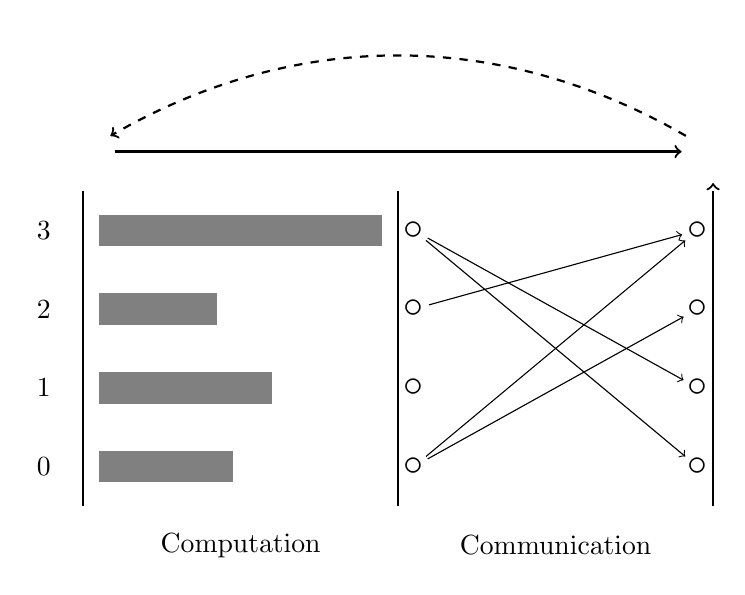
\begin{tikzpicture}[auto, node distance=1.4cm]

\node at (-0.5, 0.5) {0};
\node at (-0.5, 1.5) {1};
\node at (-0.5, 2.5) {2};
\node at (-0.5, 3.5) {3};

\draw[-, thick] (0, 0) -- (0, 4);

\fill[color=gray] (0.2, 0.3) rectangle (1.9, 0.7);
\fill[color=gray] (0.2, 1.3) rectangle (2.4, 1.7);
\fill[color=gray] (0.2, 2.3) rectangle (1.7, 2.7);
\fill[color=gray] (0.2, 3.3) rectangle (3.8, 3.7);

\draw[-, thick] (4.0, 0) -- (4.0, 4);

\draw[->, shorten >= 0.2cm, shorten <= 0.2cm] (4.2, 0.5) -- (7.8, 2.5);
\draw[->, shorten >= 0.2cm, shorten <= 0.2cm] (4.2, 0.5) -- (7.8, 3.5);
\draw[->, shorten >= 0.2cm, shorten <= 0.2cm] (4.2, 2.5) -- (7.8, 3.5);
\draw[->, shorten >= 0.2cm, shorten <= 0.2cm] (4.2, 3.5) -- (7.8, 0.5);
\draw[->, shorten >= 0.2cm, shorten <= 0.2cm] (4.2, 3.5) -- (7.8, 1.5);

\node[] at (4.2, 0.5) {\Large $\circ$};
\node[] at (4.2, 1.5) {\Large $\circ$};
\node[] at (4.2, 2.5) {\Large $\circ$};
\node[] at (4.2, 3.5) {\Large $\circ$};

\node[] at (7.8, 0.5) {\Large $\circ$};
\node[] at (7.8, 1.5) {\Large $\circ$};
\node[] at (7.8, 2.5) {\Large $\circ$};
\node[] at (7.8, 3.5) {\Large $\circ$};

\draw[-, thick] (8.0, 0) -- (8.0, 4);


\node at (2, -0.5) {Computation};
\node at (6, -0.5) {Communication};

\draw[->, thick, shorten <= 0.4 cm, shorten >= 0.4 cm] (0, 4.5) -- (8, 4.5);
\draw[->, dashed, thick, bend right, shorten <= 0.4 cm, shorten >= 0.4 cm] (8, 4.5) edge (0, 4.5);

\end{tikzpicture}

\end{document}
